\chapter{LHCとATLAS実験}\label{chapter2}
本章では、Run-3における大型ハドロン衝突型加速器であるLHC加速器とATLAS検出器の概要について述べる。


\section{LHC加速器}\label{section2-1}
LHCは周長27kmの陽子陽子衝突型大型円形加速器であり、スイスのジュネーブ郊外にあるCERN地下100mに設置されている。LHCの全体図を図~\ref{fig:2-1}に示す。LHCは重心系エネルギー\SI{14}{\tera \electronvolt}、瞬間ルミノシティ$\SI{1.0e34}{\cm^{-2}\s^{-1}}$での陽子陽子衝突が可能なように設計されている。
ルミノシティとはどれほど多くの衝突データを得られるかの指標として用いられる値で、毎秒・単位断面積当たり($\si{\cm^{-2}.\s^{-1}}$)の陽子衝突頻度である。
これを一定期間積分したものを積分ルミノシティと呼ぶ。

\begin{figure}[h]
  \centering
  \includegraphics[clip, width=11cm]{fig/2/lhc_map.jpg}
  \caption{LHC加速器の全体図\cite{article:Overall_view_LHC}。地下100mに設置されたLHCの4つ衝突点にそれぞれ検出器が配置されている。}
  \label{fig:2-1}
\end{figure}

LHCでは陽子はバンチと呼ばれる塊で2本のリングで互いに逆向きに加速され、バンチが連なることでビームを形成している。加速リング内には、超伝導電磁石によって最大8.33Tの磁場がかけられ、磁場によって陽子が曲げられ加速リング内を周回する。ビームを交差させ、25nsおきに陽子陽子衝突を起こしている。
LHCの陽子陽子衝突点は全部で4か所あり、それぞれで実験が行われている。
ATLAS~(A~Troidal~LHC~ApparatuS)、CMS~(Compact~Muon~Solenoid)\cite{article:CMSExperiment}は大型汎用検出器で、標準模型の精密測定や新物理の探索など幅広い物理を対象とした研究を行っている。
LHCb~(Large~Hadron~COllider-b)\cite{article:LHCbExperiment}はビームライン付近に感度を持つ検出器を設置することでbクォークの物理を対象とした研究を行っている。ALICE~(A~Large~Ion~Collider~Experiment)\cite{article:ALICEExperiment}は重イオンを用いた衝突実験で、鉛などの原子核を加速させ、高エネルギー領域での衝突によって生じるクォーク・グルーオンプラズマを対象とした研究を行っている。
CERNに設置されている加速器・検出器群を図~\ref{fig:2-2}に示す。

\begin{figure}[H]
  \centering
  \includegraphics[clip, width=11cm]{fig/2/accel_complex-v2022_complex.png}
  \caption{CERNに設置されている加速器・検出器群\cite{article:accelerator-complex}}
  \label{fig:2-2}
\end{figure}


図~\ref{fig:2-3}にLHCの運転計画を示す。
LHCは第1期運転~(Run-1)として2010年から本格的に運転を開始し、7TeVから8TeVの重心系エネルギー($\sqrt{s}$)で2012年まで稼働した。最高瞬間ルミノシティは$\SI{0.77e34}{\cm^{-2}\s^{-1}}$であった。その後、2013年から2015年までのシャットダウン期間~(LS1)で加速器のアップグレードを行い、2015年から2018年までRun-2として最高瞬間ルミノシティ$\SI{2.0e34}{\cm^{-2}\s^{-1}}$、積分ルミノシティ約$\SI{150}{\femto\barn^{-1}}$で運転が行われた。2019年から再びシャットダウン期間~(LS2)となり、2022初旬まで加速器のアップグレードが行われた。2022年7月よりRun-3としてデータ取得が開始され、2025年まで重心系エネルギーを13.6TeV、瞬間ルミノシティ$\SI{2.0e34}{\cm^{-2}\s^{-1}}$で運転を行い積分ルミノシティ$\SI{350}{\femto\barn^{-1}}$のデータ取得を目指している。
また、アップグレードを経て2029年からより高いルミノシティでの高輝度LHC実験(HL-LHC)の運転を予定している。

\begin{figure}[H]
  \centering
  \includegraphics[clip, width=14cm]{fig/2/HL-LHC_Janvier2022.pdf}
  \caption{LHCの運転とアップグレード計画\cite{article:LHCDesignReport}}
  \label{fig:2-3}
\end{figure}



\section{ATLAS検出器}\label{section2-2}

ATLAS検出器は、LHCの衝突点の1つに設置された直径25m、長さ44mの円筒形の大型汎用検出器である\cite{Aad:1129811}。ATLAS 検出器の全体像を図~\ref{fig:2-4}に示す。
ATLAS実験では様々な物理を研究対象としており、陽子陽子衝突によって出てくる様々な粒子の種類やエネルギー・運動量を精密に測定できるように設計されている。
その検出器は複数の検出器を組み合わせて構成され、内側から主な検出器として内部飛跡検出器、カロリメータ、ミューオン検出器が設置されている。また、内部飛跡検出器とカロリメータの間には超伝導ソレノイド磁石、カロリメータの外側にはトロイド磁石がそれぞれ設置されている。
これらの検出器から得られる情報を組み合わせることで、粒子識別や粒子のエネルギーなどの測定を行っている。

\begin{figure}[tb]
  \centering
  \includegraphics[clip,width=12cm]{fig/2/0803012_01.jpg}
  \caption{ATLAS検出器の全体図\cite{Aad:1129811}。直径~$\SI{25}{\m}$、長さ~$\SI{40}{\m}$の円筒型で、内部飛跡検出器、カロリーメータ、ミューオン検出器などの検出器を組み合わせて様々な粒子の測定を行っている。}
  \label{fig:2-4}
\end{figure}

\subsection{ATLAS検出器における座標系}\label{section2-2-1}
検出器の座標系を~\ref{fig:2-5}に示す。
ATLAS実験では直行座標系と円筒座標系が使用されており、直交座標系では、検出器の中心を原点として、ビーム軸に沿って加速器情報から見てビームが反時計回りになる方向に$z$軸を取る。ビーム軸に垂直な平面を$x-y$平面としたときに、加速器の中心方向を正とする$x$軸及び、それに対する右手系、つまり地面に対して上向きを正とする$y$軸を設定する。円筒座標系では、ビーム軸に沿った$z$軸に対し、動径方向を$R$、ビーム軸周りの角度を方位角$\phi$、ビーム軸からの角度を極角$\theta$としている。
ATLAS検出器ではz軸が正の側をA-side、負の側をC-sideと定義している。

また、一般にハドロン散乱では衝突点から粒子が放出される方向を表すために、
\begin{equation}
    \eta=-\ln\bigg(\tan\frac{\theta}{2}\bigg)
    \label{ラピディティ}
\end{equation}
と定義される擬ラピディティ$\eta$を用いる。
ATLAS 検出器は円筒形をしており、$|\eta| < 1.05$ の側面部分をバレル領域、$|\eta| > 1.05$ の底面部分をエンドキャップ領域と呼ぶ。

\begin{figure}[tb]
  \centering
  \includegraphics[clip, width=11cm]{fig/2/coordinate.pdf}
  \caption{ATLAS検出器における座標系。}
  \label{fig:2-5}
\end{figure}

\newpage
\subsection{マグネットシステム}\label{section2-2-2}
ATLAS実験では、超伝導磁石を用いて磁場をかけることにより荷電粒子の飛跡を曲げ、その曲率を測ることで横方向運動量を測定している。超伝導磁石は2種類設置され、それらは衝突点付近で発生した荷電粒子の運動量測定のために用いられるソレノイド磁石と、ミューオンの運動量測定のために用いられるトロイド磁石である。ATLAS検出器の磁石の配置を図~\ref{fig:2-6}に示す。

\begin{figure}[h]
  \centering
  \includegraphics[clip, width=11cm]{fig/2/ATLcoilGeom.pdf}
  \caption{ATLAS検出器における超電導磁石の配置。}
  \label{fig:2-6}
\end{figure}

磁石全体の大きさは半径$\SI{22}{\m}$、全長$\SI{26}{\m}$である。
ソレノイド磁石は内部検出器とカロリーメータの間に設置されており、内径$\SI{2.46}{\m}$、外径$\SI{2.56}{\m}$、z軸方向の長さ$\SI{5.8}{\m}$の円筒形である。内部の磁場は\SI{2}{\tesla}で、内部検出器中で荷電粒子の飛跡を$\phi$方向に曲げて横運動量の測定を行う。
また、トロイド磁石はカロリメータの外側に設置されている。1つのバレルトロイドとA-side、C-side両側にそれぞれ1つずつのエンドキャップトロイドで構成され、それらがビーム軸に対して8回対称になるように配置されている。バレルトロイドは内径$\SI{9.4}{\m}$、外径$\SI{20.1}{\m}$、z軸方向の長さ$\SI{25.3}{\m}$で、エンドキャップトロイドは内径$\SI{1.65}{\m}$、外径$\SI{10.7}{\m}$、z軸方向の長さ$\SI{5.0}{\m}$である。
また磁場の強さはそれぞれ、バレルトロイドでは約$\SI{0.5}{\tesla}$、エンドキャップトロイドでは約$\SI{1}{\tesla}$である。
トロイド磁石によって生じる磁場の$x-y$平面上での$r-\phi$方向と、$\eta$方向の磁場強度の分布をそれぞれ図~\ref{fig:2-7-1}、図~\ref{fig:2-7-2}で示す。

\begin{figure}[h]
  \begin{minipage}[b]{0.48\linewidth}
      \centering
      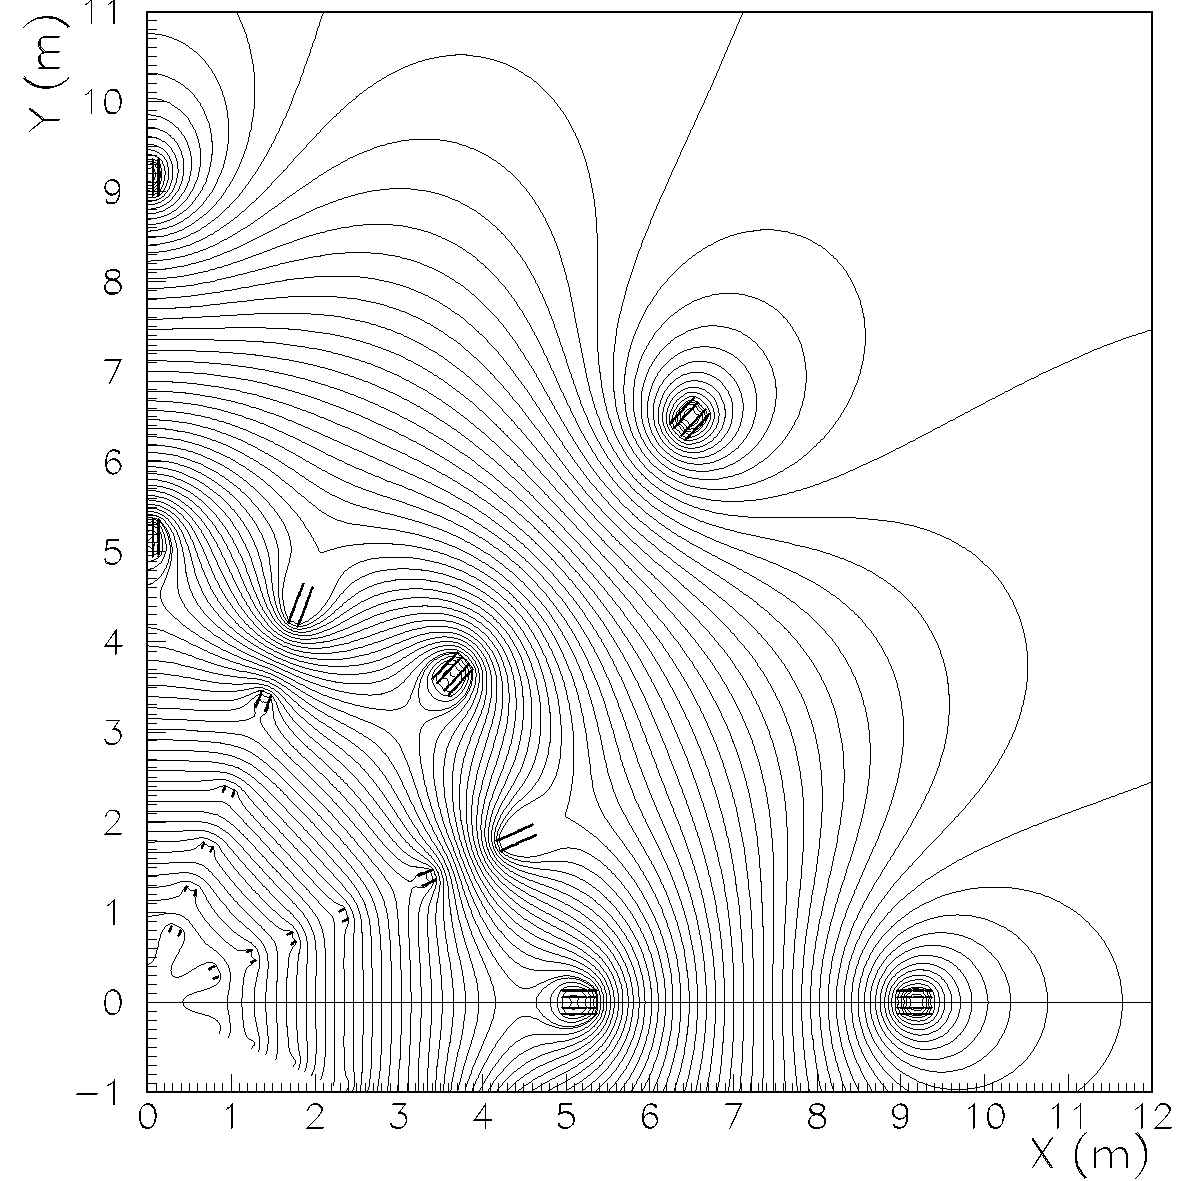
\includegraphics[clip, width=6cm]{fig/2/FMBmap.pdf}
      \subcaption{ビーム軸に対して垂直な$x-y$平面におけるトロイド磁石による磁場の$\phi$分布。}
      \label{fig:2-7-1}
  \end{minipage}
    \begin{minipage}[b]{0.48\linewidth}
      \centering
      \includegraphics[clip, width=6cm]{fig/2/bdl_cut.png}
      \subcaption{$\eta$方向の磁場強度の分布。}
      \label{fig:2-7-2}
  \end{minipage}
  \caption{超電導磁石による磁場分布\cite{article:ATLASMagneticField}。}
\end{figure}

\subsection{内部飛跡検出器}\label{2-2-3}
内部飛跡検出器は内側から~Insertable~B~Layer~(IBL)、Pixel検出器、Semi-Conductor~Tracker~(SCT)、Transition~Radiation~Tracker~(TRT)で構成される。バレル領域とエンドキャップ領域における内部飛跡検出器の配置をそれぞれ図~\ref{fig:2-8-1}、図~\ref{fig:2-8-2}に示す。
内部飛跡検出器は半径約$\SI{1.1}{\m}$、$z$軸方向に長さ約$\SI{5.3}{\m}$で、$|\eta|<2.5$の領域を覆っている。
検出器内には、前述のとおりソレノイド磁石によって約2Tの磁場がかかっており、磁場領域を通過した荷電粒子の飛跡の$\phi$方向の曲率から運動量を計算する。

\begin{figure}[h]
  \begin{minipage}[b]{0.48\linewidth}
      \centering
      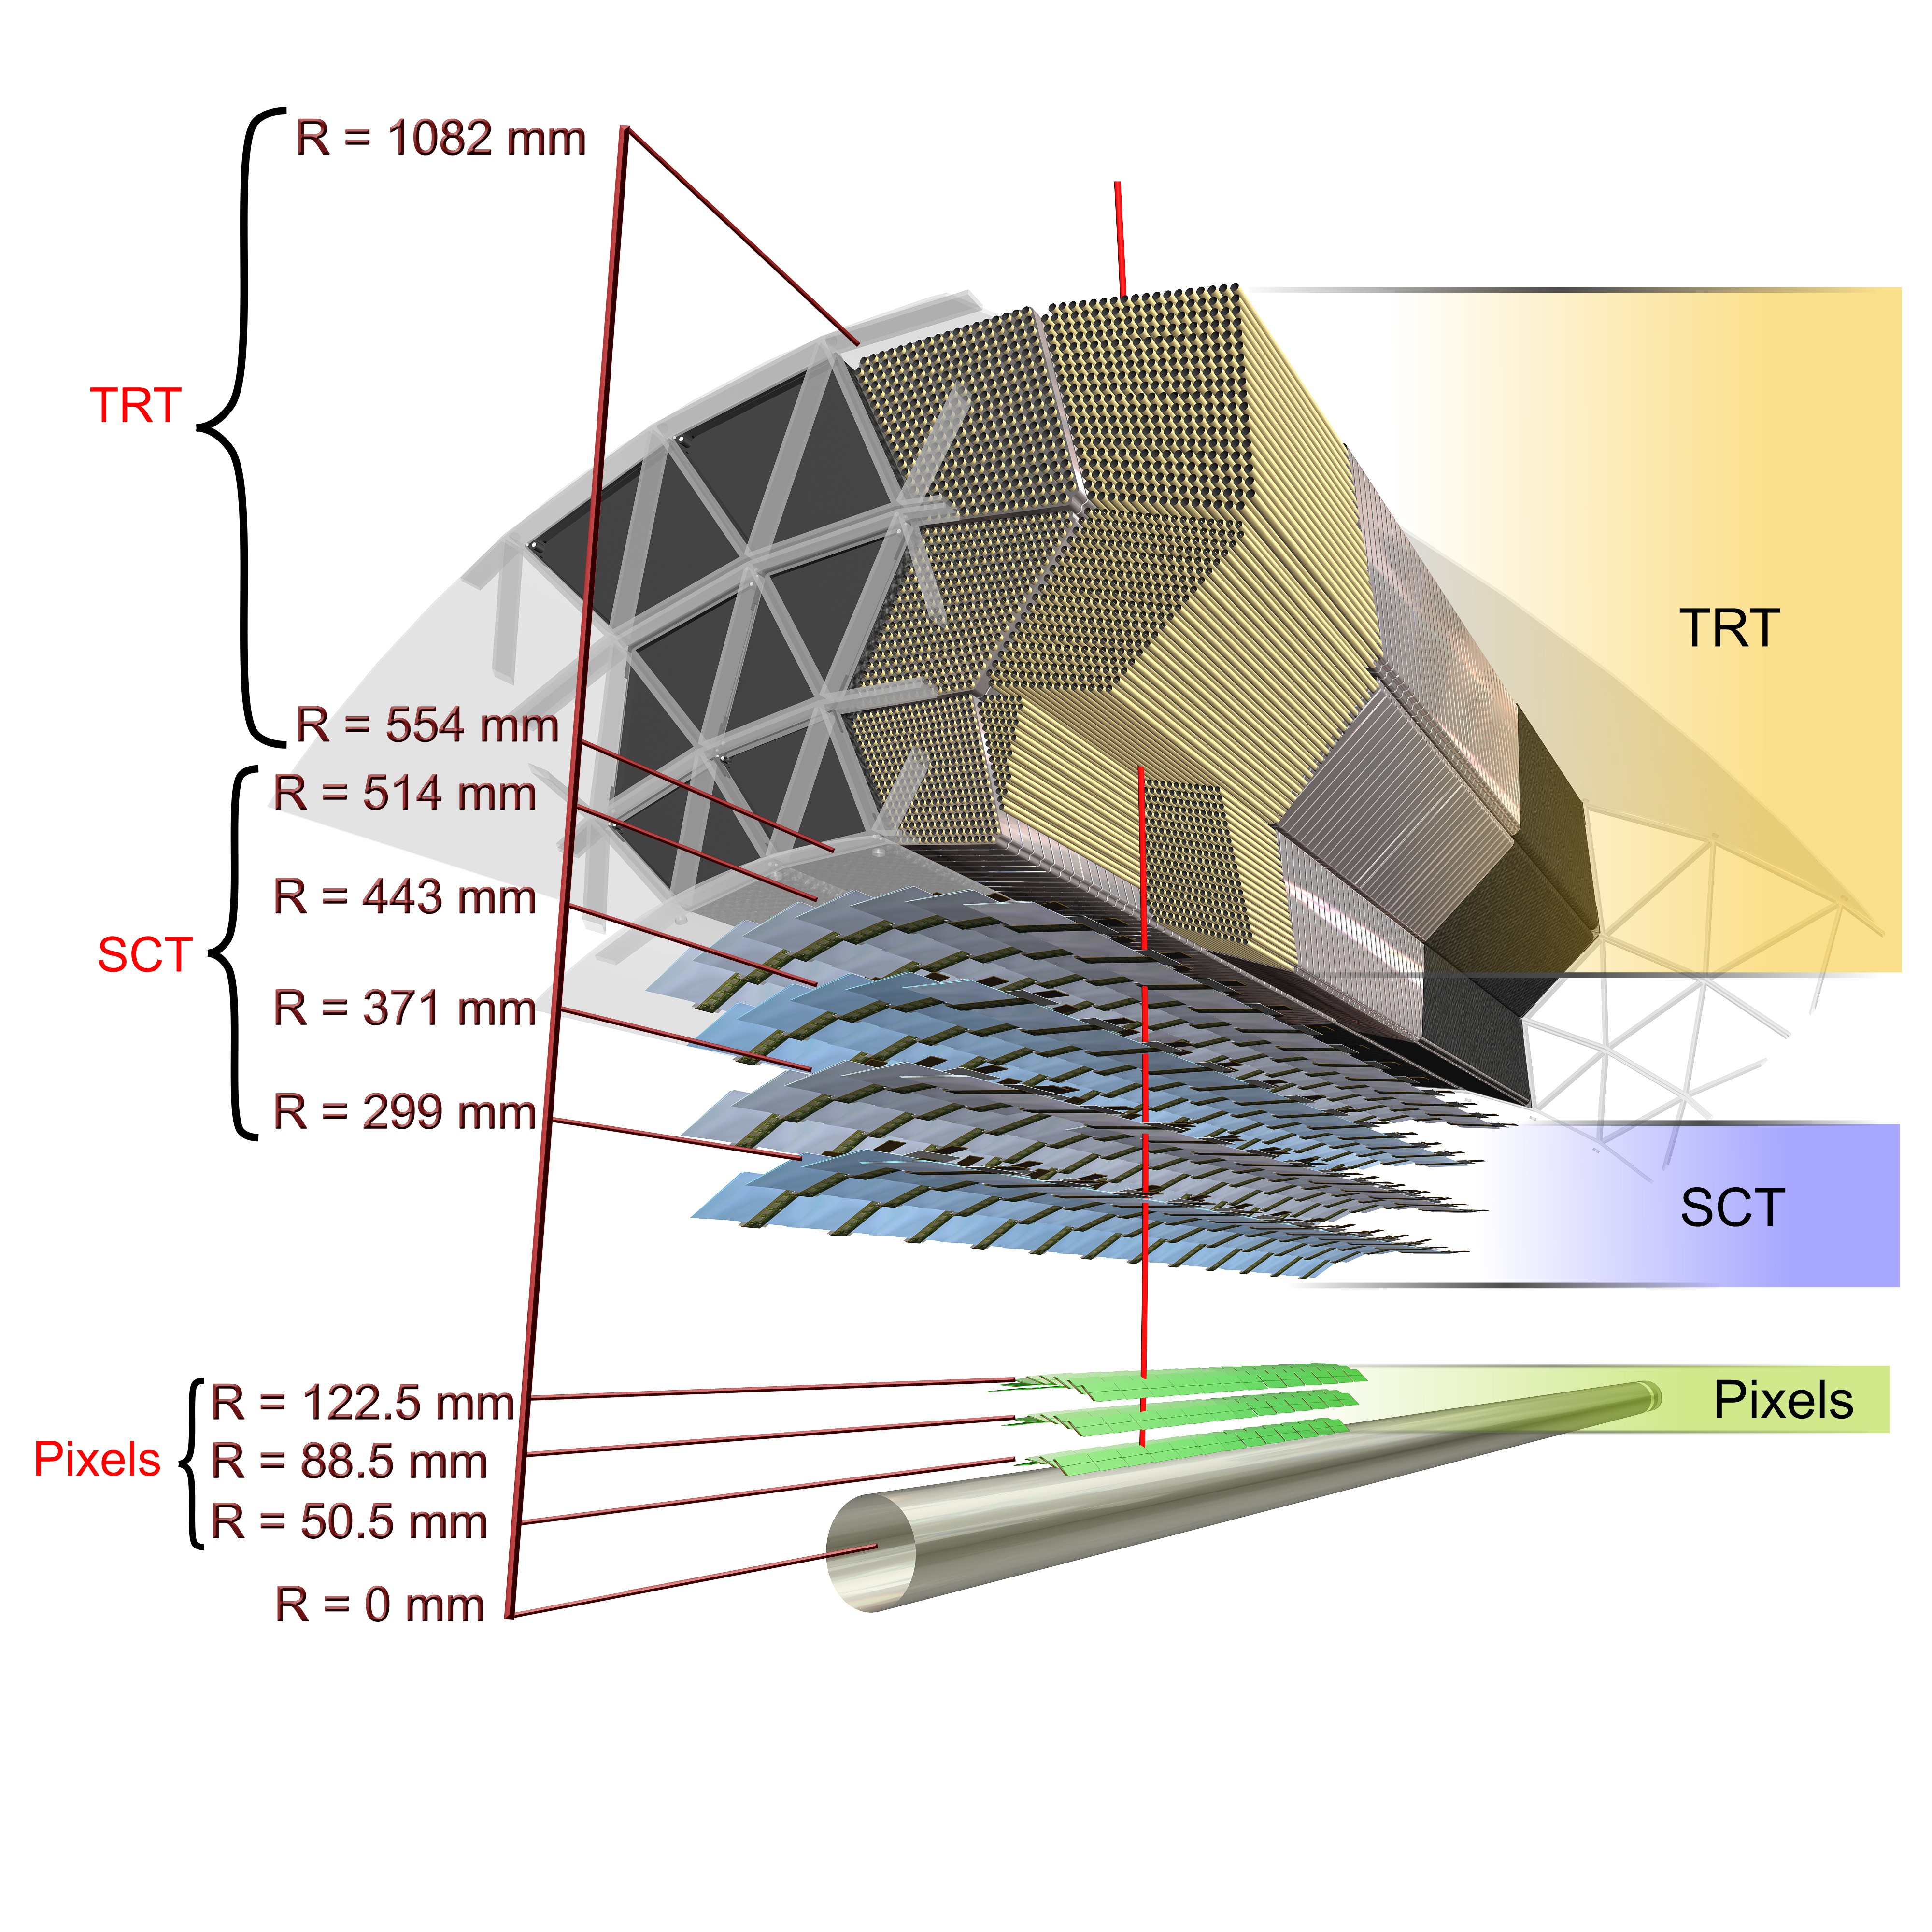
\includegraphics[clip, width=6cm]{fig/2/inner_detector2.jpg}
      \subcaption{バレル領域}
      \label{fig:2-8-1}
  \end{minipage}
    \begin{minipage}[b]{0.48\linewidth}
      \centering
      \includegraphics[clip, width=6.5cm]{fig/2/inner_detector3.png}
      \subcaption{エンドキャップ領域}
      \label{fig:2-8-2}
  \end{minipage}
  \caption{バレル領域とエンドキャップ領域での内部飛跡検出器の構造\cite{Aad:1129811}。}
\end{figure}

\subsubsection{Pixel検出器とIBL}
Pixel検出器はバレル領域で同心円状に3層、エンドキャップ領域のA-side、C-side両側にそれぞれディスク状に3層設置されている。1つのpixelサイズは$\SI{50}{\um} \times \SI{400}{\um}$で、R$\phi$方向及び$z$方向に並べて配置している。
pixel検出器の位置分解能は、R$\phi$方向に$\SI{10}{\um}$、$z$方向に$\SI{115}{\um}$である。

また、IBLは~Run-2からルミノシティ増加への対応とPixel検出器の性能向上のためにPixel検出器よりも内側に配置された。1つのpixelのサイズは$\SI{50}{\um} \times \SI{250}{\um}$で、位置分解能はR$\phi$方向に$\SI{10}{\um}$、$z$方向に$\SI{70}{\um}$である。IBLにより、ビーム軸と飛跡の最近接距離である~impact~Parameterの測定精度が改善された。

\begin{figure}[h]
  \centering
  \includegraphics[clip, width=9.5cm]{fig/2/IBL_layout.png}
  \caption{IBLのレイアウト~\cite{article:ATLASBlayerTDR}。}
  \label{fig:2-9}
\end{figure}

\subsubsection{SCT}
SCTはバレル領域で4層からなる同心円状のシリンダ形状で設置されており、エンドキャップ領域でA-side、C-sideそれぞれ9枚ずつのディスク形状になっている。
SCTの位置分解能はバレル領域でR方向に$\SI{17}{\um}$、$\phi$方向に$\SI{580}{\um}$、エンドキャップ領域ではR方向に$\SI{17}{\um}$、$z$$\SI{580}{\um}$である。


\subsubsection{TRT}
TRTはドリフトチューブを積み重ねるように構成されており、$|\eta|<2.0$の領域を覆っている。バレル領域では長さ$\SI{144}{\cm}$のチューブをビーム軸と平行に、エンドキャップ領域では長さ$\SI{37}{\cm}$のチューブを放射状に配置している。TRTの位置分解能はR-$\phi$方向に$\SI{130}{\um}$である。

また、TRTでは荷電粒子が誘電率の異なる物質へ入射する際に光子を放出する「遷移放射」を利用した電子の同定も行っている。遷移放射で放出される光子のエネルギーは粒子のローレンツ因子$\gamma$に比例するため、これを利用することで入射した荷電粒子が電子かどうか判定している。

\subsection{カロリメータ}\label{2-2-4}
カロリメータは内部飛跡検出器の外側に設置されており、内側から電磁カロリメータ、ハドロンカロリメータの順に配置されている。電磁カロリメータは電磁相互作用による電磁シャワーを用いて電子と光子のエネルギーを測定し、ハドロンカロリメータは強い相互作用によるハドロンシャワーを用いてハドロンのエネルギー測定やそれを組み合わせたジェット再構成に用いられる。ATLAS検出器におけるカロリメータの概要図を図~\ref{fig:2-10}に示す

\begin{figure}[h]
  \centering
  \includegraphics[clip, width=9cm]{fig/2/Calorimeter_d3.pdf}
  \caption{カロリメータの全体図~\cite{Aad:1129811}。}
  \label{fig:2-10}
\end{figure}

\subsubsection{電磁カロリメータ}
電磁カロリメータはバレル領域をカバーするように$|\eta|<1.5$にバレル電磁カロリメータ、エンドキャップ領域をカバーするように$1.4<|\eta|<3.2$にエンドキャップ電磁カロリメータが配置されている。
それぞれの厚さは、バレル領域で放射長の22倍以上、エンドキャップ領域で放射長の24倍以上である。
電磁カロリメータは$\phi$方向の不感領域をなくすために鉛の吸収体と強い放射線耐性を持つ液体アルゴンをアコーディオン状に組み合わせた構造になっている(図~\ref{fig:2-11})。


\begin{figure}[h]
  \centering
  \includegraphics[clip, width=9cm]{fig/2/electoricCal.jpg}
  \caption{電磁カロリメータの構造~\cite{Aad:1129811}。}
  \label{fig:2-11}
\end{figure}

\subsubsection{ハドロンカロリメータ}
ハドロンカロリメータは、電磁カロリメータと同様にバレル領域をカバーするために$|\eta|<1.7$、エンドキャップ領域をカバーするために$1.5<|\eta|<3.2$に配置されている。
バレル領域では、鉄の吸収体とシンチレータを交互に重ねたタイルカロリメータ(図~\ref{fig:2-12-1})が設置されている。シンチレーション光を波長変換ファイバーで集め、光電子増倍管で読み出しを行っている。
エンドキャップ領域では、銅の吸収体と液体アルゴンから構成されたハドロンエンドキャップカロリメータ(図~\ref{fig:2-12-2})が使用されている。
バレル領域とエンドキャップ領域に加えて、$3.1<|\eta|<4.9$のフォワード領域をカバーするために銅とタングステンの吸収体と液体アルゴンから構成されたフォワードカロリメータが設置されている。

\begin{figure}[h]
  \begin{minipage}[b]{0.45\linewidth}
      \centering
      \includegraphics[clip, width=6cm]{fig/2/TileCalo.png}
      \subcaption{Tileカロリメータ}
      \label{fig:2-12-1}
  \end{minipage}
    \begin{minipage}[b]{0.45\linewidth}
      \centering
      \includegraphics[clip, width=6cm]{fig/2/HadronEndcapCal.png}
      \subcaption{エンドキャップ領域におけるカロリメータ}
      \label{fig:2-12-2}
  \end{minipage}
  \caption{バレル領域とエンドキャップ領域でのハドロンカロリメータの構造\cite{Aad:1129811}。}
\end{figure}


\subsection{ミューオン検出器}\label{section2-2-5}
ミューオン検出器はATLAS検出器の一番外側に配置されており、カロリメータから出てきた荷電粒子の位置や横方向運動量を測定する。
ミューオン検出器は、位置分解能が高く精密測定用として用いられる検出器と、位置分解能は高くないが応答を早くして主にトリガー用として用いる検出器がある。
精密測定用の検出器は~Monitored~Drift~Tube~(MDT)、トリガー用の検出器は~Resistive~Plate~Chamber~(RPC)とThin~Gap~Chamber~(TGC)である。
またRun-3からエンドキャップ領域の磁場領域より内側に設置されていた~Small~Wheelに代わって~New~Small~Whell~(NSW)が導入された。
図~\ref{fig:2-13}にミューオン検出器の全体図を示す。

\begin{figure}[h]
  \centering
  \includegraphics[clip, width=9cm]{fig/2/muondetector.pdf}
  \caption{ミューオン検出器の全体図~\cite{Aad:1129811}。バレル領域にRPC、MDT、エンドキャップ領域にTGC、MDTが配置されている。}
  \label{fig:2-13}
\end{figure}

ミューオン検出器では、各検出器をステーションと呼ばれる層状にまとめている。これらのステーションはバレル領域とエンドキャップ領域でそれぞれ3層あり、衝突点に近い方からインナーステーション~(I)、ミドルステーション~(M)、アウターステーション~(O)と呼ばれる。バレル領域ではビーム軸周りに半径約5m、7m、10mのところに同心円状にステーションが並べられ円筒状の検出器を形成している。
エンドキャップ領域では、$|z|$が約$\SI{7.4}{\cm}$、$\SI{14}{\cm}$、$\SI{21.5}{\cm}$の位置に$z$軸に垂直にステーションが配置されており大きなホイールを形成している。また、インナーステーションとミドルステーションの間に~Endcap~Extra~(EE)と呼ばれる検出器が設置されている。

また、図~\ref{fig:2-14}で示されているように、ミューオン検出器は不感領域を失くすために$\phi$方向に大きさの違う2つのセクターを互い違いに8つずつ$\phi$方向に重ねている。2つのセクターはそれぞれ~Small~sectorと~Large~sectorと呼ばれる。
ミューオン検出器の~Large~sector、~Small~sectorの$R-z$平面の断面図を図~\ref{fig:2-15-1}、図~\ref{fig:2-15-2}に示す。

\begin{figure}[h]
  \centering
  \includegraphics[clip, width=8cm]{fig/2/muon_detector_xy.pdf}
  \caption{ミューオン検出器の$x-y$平面での断面図~\cite{Aad:1129811}。黄と橙が~Small~sector、緑と青が~Large~sector。}
  \label{fig:2-14}
\end{figure}

%-------------チェンバーの略称と検出器の対応表を書く------------------------------

\begin{figure}[h]
  \begin{minipage}[b]{0.48\linewidth}
      \centering
      \includegraphics[clip, width=6.8cm]{fig/2/muon_Rz_Large.pdf}
      \subcaption{Large~sector}
      \label{fig:2-15-1}
  \end{minipage}
    \begin{minipage}[b]{0.48\linewidth}
      \centering
      \includegraphics[clip, width=6.8cm]{fig/2/muon_Rz_small.pdf}
      \subcaption{Small~sector}
      \label{fig:2-15-2}
  \end{minipage}
  \caption{ミューオン検出器の~Large~sector、~Small~sectorの$R-z$平面の断面図\cite{article:phase2}。}
\end{figure}

\subsubsection{Monitored~Drift~Tube~(MDT)}
MDTはバレル領域、エンドキャップ領域両方に設置されており、$\SI{35}{\um}$と位置分解能が高いので精密測定に用いられる。
MDTのドリフトチューブの構造を図~\ref{fig:2-16}に示す。
MDTはArと$\rm{CO_{2}}$ガスが93 : 7の割合で充填された半径$\SI{27.979}{\mm}$のドリフトチューブで構成され、チューブの中心のワイヤーには$\SI{3080}{\V}$の電圧がかけられ電離した電子がワイヤーに集められる。
荷電粒子の通過位置は、電子のドリフト距離から求めたドリフトサークルの接線であり分解能は$R$方向、$z$方向ともに$\SI{35}{\um}$である。
また電子の最大ドリフト時間は約$\SI{700}{\ns}$である。

\begin{figure}[h]
  \centering
  \includegraphics[clip, width=8cm]{fig/2/mdt_driftTube.png}
  \caption{MDTのドリフトチューブの構造~\cite{Aad:1129811}。}
  \label{fig:2-16}
\end{figure}

MDTは図~\ref{fig:2-17}で表されるように、ドリフトチューブ4レイヤーまたは3レイヤーを2層重ねた構造になっている。
MDTはバレル領域では長方形、エンドキャップ領域では台形であり、ドリフトチューブは$\phi$方向に沿って並べられ、磁場による主な曲がり方向に対応したバレル領域で$z$方向、エンドキャップ領域で$R$方向の位置測定により運動量を測定する。

\begin{figure}[h]
  \centering
  \includegraphics[clip, width=8cm]{fig/2/MDT_chamber_schematics_2.pdf}
  \caption{MDTの構造~\cite{Aad:1129811}。}
  \label{fig:2-17}
\end{figure}

\subsubsection{Resisitive~Plate~Chamber~(RPC)}
RPCはバレル領域に設置されている、主にミューオントリガー用のガス検出器である。
構造を図~\ref{fig:2-18}に示す。2枚の高抵抗プレートの間に幅$\SI{2}{\mm}$の絶縁体が挟み込まれており、プレート間には約$\SI{4.9}{\kV/\mm}$の電場が形成されている。
プレート間には、$\rm{C_{2}H_{2}F_{4}/Iso - C_{4}H_{10}/SF_{6}(94.7 : 5 : 0.3)}$の混合ガスが充填されている。
ミューオンが通過した際に、ガスから電離した電子が電場に沿って雪崩増幅を起こし、その電荷による誘導電荷をプレートの外側に取り付けられたストリップで読み出す。
分解能は$z$方向、$\phi$方向どちらも$\SI{10}{\mm}$である。

\begin{figure}[h]
  \centering
  \includegraphics[clip, width=8cm]{fig/2/RPC_structure.pdf}
  \caption{RPC検出器の構造~\cite{Aad:1129811}。}
  \label{fig:2-18}
\end{figure}

図~\ref{fig:2-19}で表されるように、Large~sectorと~Small~sectorそれぞれに、MDTミドルステーションを挟み込むように2枚、MDTアウターステーションの外側に1枚の、計3枚のRPCが配置されている。
1枚のRPCは直交した$\eta$--stripと$\phi$--stripから構成されており、2次元での読み出しを行う。
MDTでは$\phi$方向の測定ができないので、RPCで測定した$\phi$の情報を用いる。

\begin{figure}[h]
  \centering
  \includegraphics[clip, width=8cm]{fig/2/RPC_xy.pdf}
  \caption{RPC検出器の$x-y$平面での断面図~\cite{Aad:1129811}。}
  \label{fig:2-19}
\end{figure}

\subsubsection{Thin~Gap~Chambers~(TGC)}
TGCはエンドキャップ領域に設置されている、主にミューオントリガー用のガス検出器である。
構造を図~\ref{fig:2-20}に示す。
TGCの各層は、ワイヤーとアノード層、ストリップ層から構成されているマルチワイヤーガス検出器で、$\eta$方向をワイヤー、$\phi$方向をストリップで測定している。内部には、$\rm{CO_{2}}$と$\rm{n - C_{5}H_{12}}$ガスが充填されている。
ワイヤー間の距離を$\SI{1.8}{\mm}$、ワイヤーとストリップの距離を$\SI{1.4}{\mm}$と短くすることによって高い時間分解能を実現している。
位置分解能は$\phi$方向で$3-7$~$\si{\mm}$、$R$方向で$2-6$~$\si{\mm}$である。

\begin{figure}[h]
  \centering
  \includegraphics[clip, width=8cm]{fig/2/l1mue-schema.pdf}
  \caption{TGC検出器の配置~\cite{Aad:1129811}。}
  \label{fig:2-20}
\end{figure}

図~\ref{fig:2-20}で表されるように、インナーステーションに1枚、ミドルステーションに3枚配置されている。
インナーステーションではdoublet構造1枚が2層、ミドルステーションではdoublet構造が2枚、triplet構造が1枚の合計7層から構成されている。doublet構造とtriplet構造を図~\ref{fig:2-22}に示す。
バレル領域と同様にMDTでは$\phi$方向の測定ができないので、TGCで測定した$\phi$の情報を用いる。

\begin{figure}[h]
  \centering
  \includegraphics[clip, width=8cm]{fig/2/TGC_anode_wire.pdf}
  \caption{TGC検出器の構造~\cite{Aad:1129811}。}
  \label{fig:2-21}
\end{figure}

\begin{figure}[h]
  \centering
  \includegraphics[clip, width=10cm]{fig/2/TGC_construction.pdf}
  \caption{boublet構造(左)とtriplet構造(右)~\cite{Aad:1129811}。}
  \label{fig:2-22}
\end{figure}


\subsubsection{New~Small~Wheel~(NSW)}
NSWはRun-3よりLHCのルミノシティ増加に伴う高ヒットレート状況下での飛跡測定効率の向上とミューオントリガーの改良を目的として、エンドキャップ領域の磁場領域よりも内側に、これまで~MDTと~TGCで構成されていた~Small~Wheelに代えて新たに導入された検出器である。
図~\ref{fig:2-23}に~NSWの全体図を示す。
NSWはトリガー用の~small-strip~TGC~(sTGC)と精密測定用の~MicroMegas~(MM)の2種類の検出器をそれぞれ8層ずつ組み合わせた構造をしている。
衝突点側から、sTGC~4層、MM~4層、MM~4層、sTGC~4層の順に16層配置されている。

\begin{figure}[h]
  \centering
  \includegraphics[clip, width=10cm]{fig/2/NSW_structure.png}
  \caption{NSWの全体図\cite{article:ATLASNSWTDR}。左がLarge~Station、右がSmall~Station。}
  \label{fig:2-23}
\end{figure}

sTGCの構造を図~\ref{fig:2-24}に示す。
sTGCでは$\eta$方向と$\phi$方向の測定を、それぞれストリップとワイヤーを用いて行う。
ワイヤー20本ずつがまとめて読み出され、その間隔は$\SI{1.8}{\mm}$で、ワイヤー平面から$\SI{1.4}{\mm}$の距離にある2つのカソード面に挟まれた構造になっている。
カソード面の裏には片側にはパッド、もう一方にワイヤーと垂直にストリップが配置されている。
ストリップの幅は$\SI{3.2}{\mm}$である。ストリップの幅がATLASで用いられている~TGCと比べてはるかに小さいため、位置分解能が高く~small-strip~TGCと呼ばれている。
sTGCではガスギャップを通過した荷電粒子の位置を、$\SI{150}{\um}$の位置分解能で再構成することができる\cite{article:ATLASNSWTDR}。

\begin{figure}[h]
  \centering
  \includegraphics[clip, width=9cm]{fig/2/stgc-structure.pdf}
  \caption{sTGCの構造\cite{article:ATLASNSWTDR}。}
  \label{fig:2-24}
\end{figure}

MMの構造を図~\ref{fig:2-25}に示す。
MMはドリフト電極とガスギャップ、薄い金属メッシュ、増幅領域、読み出し電極で構成されている。ガスギャップは厚さ$\SI{5}{\mm}$で、Arと$\rm{CO_{2}}$が93 : 7で混合されたガスで充填されている。
荷電粒子がMMを通過することで生じた電子がメッシュにドリフトし、メッシュを通過した後で雪崩増幅を起こし、読み出し電極に到達することで入射粒子の位置を特定する。
雪崩増幅で生じたイオンは電子と反対方向に移動し、メッシュに戻る。
ドリフト領域と増幅領域が分かれているのが~MMの大きな特徴で、増幅領域が$\SI{100}{\um}$と他の検出器に比べて非常に狭くイオンの回収を非常に高速でできるため、高ヒットレート下での読み出しに適した検出器である。
また、$\SI{450}{\um}$ピッチの読み出し電極による高精度位置測定も~MMの利点である。R方向に$\SI{100}{\um}$以下の位置分解能を持つ~\cite{article:ATLASNSWTDR}。
%NSW TDRより、SWに代わる検出器への要求?

MMは1つの~sectorに8層設置されるが、2次元読み出しを可能にするために4層でストリップを底面に平行に、残りの4層では$\pm \si{\ang{1.5}}$ずつ傾けて配置している(図~\ref{fig:2-26})。並行な層を~X層、傾けて配置された層を~U~(V)層と呼ぶ。

\begin{figure}[h]
  \centering
  \includegraphics[clip, width=13cm]{fig/2/mm-structure.pdf}
  \caption{MMの構造\cite{article:ATLASNSWTDR}。}
  \label{fig:2-25}
\end{figure}

\begin{figure}[h]
  \centering
  \includegraphics[clip, width=11cm]{fig/2/mm_stereolayer.png}
  \caption{MM$y−z$平面におけるX,U,V 層の並びと$x−y$平面で見た各層のストリップの配置\cite{article:kumaoka}。}
  \label{fig:2-26}
\end{figure}